\documentclass[wide,a4paper,titlepage,12pt] {article}
\usepackage{polski}
\usepackage{float}
\usepackage[utf8]{inputenc}
\usepackage{listings}
\usepackage{slashbox}
\usepackage[table]{xcolor}
\usepackage{graphicx,pdflscape}
\usepackage{placeins}


\title{Technologie sieciowe 2}
\author{Tymon Tobolski (181037)\\ Jacek Wieczorek (181043)}

% Title page layout (fold)
\makeatletter
\renewcommand{\maketitle}{
\begin{titlepage}
  \begin{center}
    \vspace*{3cm}
    \LARGE \@title \par
    \vspace{2cm}
    \textit{\small Autor:}\par
    \normalsize \@author\par \normalsize
    \vspace{3cm}
    \textit{\small Prowadzący:}\par
    Dr inż. Arkadiusz Grzybowski\par
    \vspace{2cm}
    Wydział Elektroniki\\ III rok\\ Pn TN 11.15 - 13.00\par
    \vspace{4cm}
    \small \@date
  \end{center}
\end{titlepage}
}
\makeatother


\begin{document}
\maketitle
  \section{Cel laboratorium}
  \paragraph{}
  Celem laboratorium było opanowanie umiejętności konfiguracji sieci VLAN oraz łącza typu trunk w oparciu o protokól IEEE 802.1q na przełącznikach Cisco 2900.

  \section{Zadania}

  \subsection{Zestawienie sieci}
  \paragraph{}
  Zadanie polegało na zestawieniu sieci składającej się z jednego przełącznika oraz dwóch stacji roboczych.
  Z przydzielona puli adresów \textbf{10.4.0.64/27} stacje robocze otrzymały następujące adresy: PC1 - \textbf{10.4.0.66/27} oraz PC2 - \textbf{10.4.0.67/27}.
  \paragraph{}
  Stacje robocze zostały podłączone do przełącznika kablami prostymi.

  Połączenie między stacjami zostało zweryfikowane przy użyciu programu \textbf{ping}.

  \begin{figure}[H]
    \begin{center}
      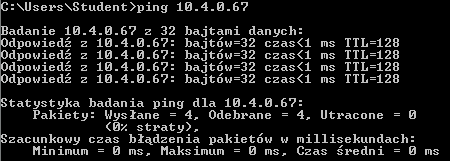
\includegraphics[width=\textwidth]{img/j1.PNG}
      \caption{Weryfikacja połączenia między stacją PC1 a PC2}
    \end{center}
  \end{figure}

  \begin{figure}[H]
    \begin{center}
      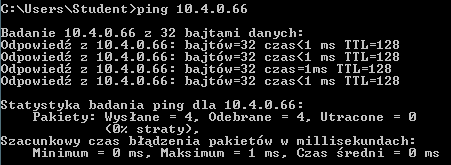
\includegraphics[width=\textwidth]{img/t1.PNG}
      \caption{Weryfikacja połączenia między stacją PC2 a PC1}
    \end{center}
  \end{figure}

  \subsection{Podłączenie portu konsolowego}
  \paragraph{}
  Przełącznik został podłączony za pomocą kabla rollover do stacji roboczej PC2.

  Obecna konfiguracja przełącznika została usunięta za pomocą komend:
  \begin{verbatim}
    delete flash:vlan.dat
    erase startup-config
    reload
  \end{verbatim}

  Nazwa przełącznika (\textbf{S1}) została zmieniona za pomocą komendy:
  \begin{verbatim}
    hostname S1
  \end{verbatim}


  \begin{figure}[htbp]
    \begin{center}
      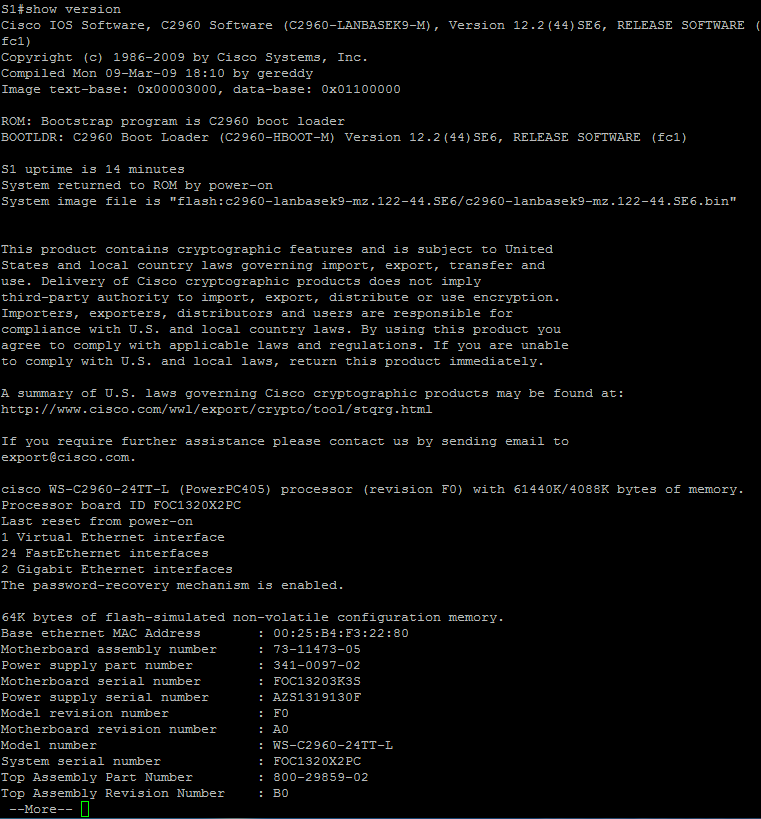
\includegraphics[width=\textwidth]{img/t3.PNG}
      \caption{Wynik polecenia $show\ version$}
    \end{center}
  \end{figure}

  \begin{figure}[htbp]
    \begin{center}
      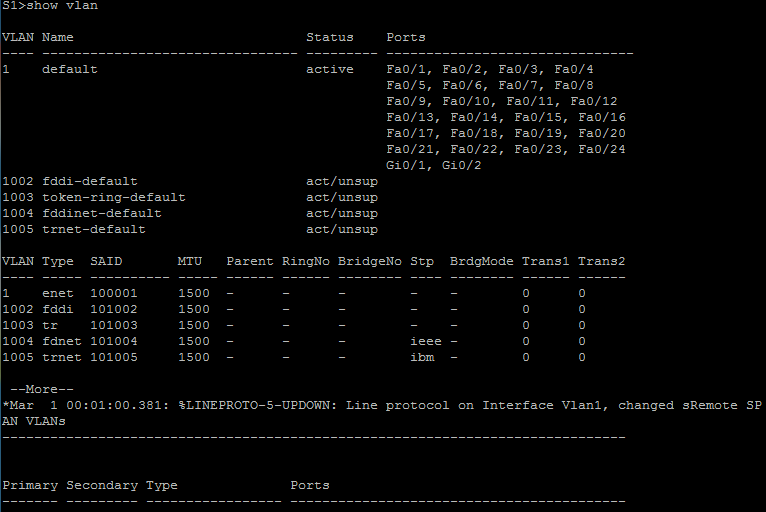
\includegraphics[width=\textwidth]{img/t4.PNG}
      \caption{Wynik polecenia $show\ vlan$}
    \end{center}
  \end{figure}

  \paragraph{}
  Na Rysunku 4 przedstawiona jest konfiguracja VLAN przełącznika po zresetowaniu konfiguracji startowej. Przełącznik posiada skonfigurowaną jedną sieć VLAN (domyślną), do której przypisane są wszystkie porty.


  \subsection{Tworzenie sieci VLAN}
  \paragraph{}
  W celu utworzenia dwóch sieci VLAN o nazwach \textbf{JacekWieczorek} i \textbf{TymonTobolski} na jednym przełączniku zostały wykonane następujące komendy:
  \begin{verbatim}
    S1(config)#vlan 10
    S1(config-vlan)#name JacekWieczorek

    S1(config)#vlan 11
    S1(config-vlan)#name TymonTobolski
    name
  \end{verbatim}

  \paragraph{}
  Do powstałych sieci VLAN zostały dołączone porty przełącznika według Tabeli 1.
  Poniżej znajdują się komendy użyte do przypisania portów do odpowiednich sieci.

  \begin{verbatim}
    S1(config)#interface fa0/4
    S1(config-if)#switchport mode access
    S1(config-if)#switchport access vlan 10

    S1(config)#interface fa0/7
    S1(config-if)#switchport mode access
    S1(config-if)#switchport access vlan 10

    S1(config)#interface fa0/11
    S1(config-if)#switchport mode access
    S1(config-if)#switchport access vlan 10

    S1(config)#interface range fa0/14-22
    S1(config-if)#switchport mode access
    S1(config-if)#switchport access vlan 10
  \end{verbatim}


  \begin{table}[H]
    \begin{center}
      \begin{tabular}{|c|c|c|}
      \hline
      & VLAN 2 & VLAN 3 \\
      \hline
      S1 & 4,7,11 & 14-22 \\
      \hline
      S2 & 9-21 & 1,4,7 \\
      \hline
      \end{tabular}
    \end{center}
    \caption{Pula portów VLAN}
  \end{table}



\end{document}